\chapter{Experiments}

In this chapter we present our experimental results and compare them to baseline solutions.
The most important baseline that we would like to improve upon is the standard LSA.
Further we present bag of words baseline and baseline based on neural embeddings.

To make our evaluation more robust, we perform it on multiple classification datasets and multiple classification tasks.

\section{Classification datasets}
    
    To evaluate the performance of different approaches, we make use of multiple popular datasets.
    
    In this section we describe these datasets in more details.
    
    \subsection{Overview} \label{sec:data:overview}
    
    We use datasets from  SentEval\footnote{\url{https://github.com/facebookresearch/SentEval}} repository.
    SentEval is a library for evaluating the quality of unsupervised sentence embeddings \cite{conneau2017supervised}.
    We have not directly used  any code from this library, because we were not able to modify its API in a maintainable way to fit our needs. 
    In the end we just used it as a guideline for dataset acquisition.
    Specifically, we only used the \texttt{get\_transfer\_data.bash} script.
    
    This repository contains multiple a lot of different datasets, 
    but we only use those related to binary classification tasks.
    
    We use:
    \begin{itemize}
        \item Movie review sentiment analysis dataset MR.
        \item Product review dataset CR.
        \item Subjectivity/objectivity dataset SUBJ.
        \item Question-type dataset TREC.
        \item Opinion polarity dataset MPQA.
    \end{itemize}
    
    \begin{table}[h]
    \begin{center}
    
    \begin{tabular}{l|rrrrr}
    \toprule
    {} &        CR &      MPQA &         MR &      SUBJ &      TREC \\\hline
    \midrule
    \#examples                                &   3775 &  10606 &   10662 &   10000 &   5952 \\\hline
    \#unique words                            &   5674 &   6238 &   20325 &   22636 &   8968 \\\hline
    \#words                                   &  75932 &  32779 &  230162 &  246015 &  58468 \\\hline
    \specialcell{\#words with\\$1$ apperance} &   2714 &   3117 &   10160 &   11152 &   5338 \\\hline
    \specialcell{avg sentence\\length}       &     20.11 &      3.09 &      21.59 &      24.60 &      9.82 \\\hline
    \specialcell{max sentence\\length}       &    106 &     44 &      62 &     122 &     37 \\\hline
    \specialcell{median sentence\\length}    &     18 &      2 &      21 &      23 &      9 \\\hline
    bias                                     &      0.64 &      0.69 &       0.50 &       0.50 &       NaN \\
    \bottomrule
    \end{tabular}
    
    \caption[Dataset characteristics]{Dataset characteristics}
    \label{tab:datasets:stats}
    \end{center}
    \end{table}


    In table \ref{tab:datasets:stats} we present a few basic statistics for each dataset.
    Column \emph{bias} denotes percentage of the majority class in the dataset.
    It also presents a baseline accuracy which a naive algorithm could achieve by making constant predictions. 
    Bias for TREC dataset is not applicable because this dataset is not binary and we address this in section \ref{sec:TREC}.
    
    We introduce each of these datasets in more details and we provide some example sentences from these datasets.
    Note, that these examples are displayed in a very genuine way. 
    We see these examples as they really are and as they are presented to our algorithms.
    The actual preprocessing will be discussed later in this section.
    
    \subsubsection{Movie review, MR}
    
    With rise of internet forums and critique websites arose a problem of sentiment classification.
    
    This dataset contains movie reviews from site Rotten Tomatoes collected by Bo Pang and Lillian Lee \cite{pang2002thumbs}.
    Originally each comment is accompanied by categorical rating with values ``fresh'' (good movie) to ``rotten'' (bad movie). 
    These labels were transformed into this freely available dataset\footnote{\url{http://www.cs.cornell.edu/people/pabo/movie-review-data/}}.
    
    Example of positive review in this dataset is: \emph{the rock is destined to be the 21st century 's new conan and that he 's going to make a splash even greater than arnold schwarzenegger , jean-claud van damme or steven segal .}

    Example of an negative review: \emph{simplistic , silly and tedious .}
    
    \subsubsection{Product review, CR}
    
    This dataset was introduced by Hu and Liu \cite{hu2004mining} as a part of a customer review summarization task. 
    They created a summarization pipeline with multiple steps and adressed a lot of different problems. 
    
    We are only interested in the sentiment prediction part, where they present a novel product review dataset.
    
    Example of a positive review:
    \emph{im a more happier person after discovering the i/p button ! .}

    Example of a negative review:
    \emph{weaknesses are minor : the feel and layout of the remote control are only so-so ; . it does n 't show the complete file names of mp3s with really long names ; . you must cycle through every zoom setting ( 2x , 3x , 4x , 1/2x , etc . ) before getting back to normal size [ sorry if i 'm just ignorant of a way to get back to 1x quickly ] .}

    \subsubsection{Opinion polarity MPQA}

    Another sentiment dataset collected by Wiebe \cite{wiebe2005annotating}.
    Its focus is to capture not only the overall tone of the document but also strength of the tone.
    However we will use only the binary positive-negative classification.
    Wiebe designed a fine grained annotation scheme and employed it on sentence corpus of articles from the world press.
    
    Example of a positive sentence:
    \emph{are also being encouraged}
    
    Example of a negative sentence:
    \emph{failing to support} 

    
    \subsubsection{Question-type, TREC}\label{sec:TREC}
    
    An important step in question answering and other dialog systems is to classify the question to the anticipated type of the answer. 
    For example, the question of \emph{Who is a good boy?} should be classified into the type of animal (entity), because the question probably refers to some dog.  
    This information would narrow down the search space to identify the correct answer string \cite{huang2008question}. 
    
    This dataset contains questions and their labels in such classification.
    There are $6$ labels: 
    
    \begin{itemize}
        \item abbreviation (ABR): \emph{what is the full form of .com?}
        \item description (DESC): \emph{how did serfdom develop in and then leave russia?}
        \item entity (ENTY): \emph{what films featured the character popeye doyle?}
        \item human (HUM): \emph{what contemptible scoundrel stole the cork from my lunch?}
        \item location (LOC): \emph{what sprawling u.s. state boasts the most airports?}
        \item numeric (NUM): \emph{when was ozzy osbourne born?}
    \end{itemize}
    
    As can be seen, this dataset is not binary. 
    For our purposes, we create $6$ different binary datasets out of this one by employing \emph{one-vs-all} strategy (one-vs-the-rest) used while training prediction models.
    This strategy consists in fitting one classifier per class. 
    For each classifier, the class is fitted against all the other classes. 
    Hence new dataset TREC-ABR will contain the same samples, but labels will be binary, $1$ if the sentence was originally in class ABR and $0$ otherwise.
    
    \begin{table}[h]
    \begin{center}
    
    \begin{tabular}{lrrrrrr}
    \toprule
    {} &  ABBR &  DESC &  ENTY &   HUM &   LOC &   NUM \\
    \midrule
    bias &  0.98 &  0.78 &  0.77 &  0.78 &  0.85 &  0.83 \\
    \bottomrule
    \end{tabular}
    
    \caption[TREC subtasks characteristics]{TREC subtasks characteristics}
    \label{tab:trec:stats}
    \end{center}
    \end{table}

    \subsubsection{Subjectivity/objectivity, SUBJ}
    
    There is number of sub-tasks that can help in context of sentiment prediction.
    One such task is to decide whether the text was subjective or objective.
        
    Pang and Lee were able to mine the Web and create a large, automatically labeled sentence corpus. 
    To gather subjective sentences they collected movie review snippets from website  \url{www.rottentomatoes.com}.
    To obtain objective data, they took sentences from plot summaries available from the Internet Movie Database \url{www.imdb.com}\footnote{We personally think, that this technique is rather questionable at best, because the labels are probably very noisy.} \cite{pang2004sentimental}.
    
    Example of a objective review:
    \emph{the movie begins in the past where a young boy named sam attempts to save celebi from a hunter .}

    Example of a subjective review:
    \emph{smart and alert , thirteen conversations about one thing is a small gem .}
    

    \subsubsection{Preprocessing} \label{sec:preprocessing}
    
    Examples provided for each dataset could be slightly strange at the first glance.
    We deliberately did only minimal processing in terms of word filtering and normalization.
    The datasets are already tokenized, we only lower-case the text.
    We do not filter any stop words (\texttt{the}) or non token characters (like question marks \texttt{?}). 
    Not filtering words that are generally filtered showed to be an important decision that allowed us to get an insight from data.
    
    LSA is commonly accompanied by heavy filtering and it is known, that stop words removal helps the performance.
    Our rational behind minimal filtering is, that we would like the weighting scheme to understand, which words are important.
    Hence we hope, that if the stop word is really not important, its weight will be reduced.
    
    \subsection{Evaluation metrics}
    
    Because we deal with binary classification tasks, our metric of choice is an accuracy.
    
    Accuracy of our $p$ predictions $\hat{y}$ given the true labels $y$ can be computed as
    $$acc_y(\hat{y}) = \frac{1}{p}\sum_{i=1}^py_i ==\hat{y}_i$$
    
    Note that this metric can have problems with unbalanced datasets. 
    We just need to remember, that what is a good accuracy depends on the dataset.
    For example accuracy $0.69$ on MPQA dataset is really bad, because it can be achieved by constant classifier.
    To address this issue, we usually subtract this baseline from our results and look only on the relative improvement. 
    
    We will compute accuracy on three subsets of the dataset. 
    $\mathrm{acc}_{train}$ on the train set, $\mathrm{acc}_{valid}$ on the validation set and $\mathrm{acc}_{test}$ on the test set.
    Note that $\mathrm{acc}_{train}$ is not very interesting on its own, but if we compare it with $\mathrm{acc}_{valid}$ and $\mathrm{acc}_{test}$ we can get an insight about whether our model is overfitting or underfitting.


\section{Baselines} \label{sec:baseline}

    There is a number of baselines that we consider.
    These are commonly used approaches such as pretrained neural embeddings, or very naive baselines such as constant classifier.
    
    To  address the problems of accuracy as a metric, we report relative improvements over the bias of each dataset.
    This can be viewed as an improvement over the precision of the constant classifier, but it is slightly more stable in this way. 
    For absolute accuracies refer to the appendix \ref{appendix:detailed}. 

    The most important baseline we want to improve upon is in section \ref{sec:lsa:baseline}, 
    and it is the standard LSA.

    \subsection{Constant baselines}
    
    As discussed in section \ref{sec:data:overview}, some of our datasets are biased. 
    They may contain substantially more examples belonging to one label that belonging to the other.
    Because of this, we can ``train'' a very simple constant classifier. 
    This classifier counts number of samples in each class in the training set and than always outputs the majority class.
    
    We do not include the result table for this classifier it is almost identical to the bias of given dataset.
    There are minor differences (on 3rd or 4th decimal place) because of the random data split. 

    \subsection{Bag of word baselines}
    
    First we evaluate baselines that work with local word representation (section \ref{sec:local:representation}).
    These baselines have no knowledge about semantic properties of words and usually only captures some basic word statistic.
    They are usually the first pick for any task, because they are simple and easy to use. 
    
    \subsubsection{Logistic regression}
    
    First commonly used baseline is a BOW representation with logistic regression as a classifier. 
    We test multiple different supervised and unsupervised word weighting schemes.
    
    It could be argued, that using term weights is not necessary when using logistic regression as the classifier.
    The argument is, that the term weighs could in theory be absorbed into the weights of the classifier. 
    This argument is actually true if we only consider the TF part of the weighting scheme.
    
    However, this argument only holds for the optimal solution. 
    The problem is, that even though an equivalent solution exists, it may not be found by the learning algorithm. 
    In practice it is useful to add the weighting scheme, 
    as it introduces some form of knowledge (a bias), 
    because we tell then the algorithm which words are probably more important.
    Because of that we may employ more strict regularization techniques without significant decrees in the performance.
    


\begin{table}[H]
\begin{center}

\begin{tabular}{llrrrr}
\toprule
{} &      &  CR &  MPQA &  MR &  SUBJ \\
scheme &  &            &              &            &              \\
\midrule
None & test &      0.150 &        0.150 &      0.261 &        0.407 \\
{} & train &      0.333 &        0.224 &      0.477 &        0.495 \\
tfchi2 & test &      0.114 &        0.119 &      0.184 &        0.336 \\
{} & train &      0.151 &        0.167 &      0.206 &        0.345 \\
tfgr & test &      0.109 &        0.125 &      0.168 &        0.340 \\
{} & train &      0.151 &        0.168 &      0.209 &        0.345 \\
tfidf & test &      0.134 &        0.150 &      0.247 &        0.404 \\
{} & train &      0.362 &        0.291 &      0.500 &        0.500 \\
tfig & test &      0.131 &        0.127 &      0.175 &        0.339 \\
{} & train &      0.152 &        0.167 &      0.212 &        0.347 \\
tfor & test &      0.154 &        0.150 &      0.269 &        0.408 \\
{} & train &      0.255 &        0.198 &      0.403 &        0.436 \\
tfrf & test &      0.125 &        0.139 &      0.228 &        0.384 \\
{} & train &      0.200 &        0.181 &      0.323 &        0.419 \\
\bottomrule
\end{tabular}

\caption[Accuracy improvements for BOW baseline]{Accuracy improvements for BOW baseline}
\label{}
\end{center}
\end{table}



\begin{table}[H]
\begin{center}

\begin{tabular}{llrrrrrr}
\toprule
{} &&  ABBR &  DESC &  ENTY &  HUM &  LOC &  NUM \\
scheme &  & & & &&&\\
\midrule
None & test & 0.011 & 0.144 & 0.100 &0.137 &0.114 &0.128 \\
{} & train & 0.011 & 0.199 & 0.209 &0.203 &0.141 &0.159 \\
tfchi2 & test & 0.009 & 0.097 & 0.014 &0.115 &0.099 &0.093 \\
{} & train & 0.009 & 0.091 & 0.013 &0.112 &0.103 &0.088 \\
tfgr & test & 0.007 & 0.085 & 0.009 &0.105 &0.096 &0.094 \\
{} & train & 0.007 & 0.096 & 0.013 &0.112 &0.100 &0.095 \\
tfidf & test & 0.007 & 0.144 & 0.110 &0.146 &0.120 &0.138 \\
{} & train & 0.016 & 0.218 & 0.226 &0.216 &0.154 &0.170 \\
tfig & test & 0.007 & 0.091 & 0.009 &0.104 &0.103 &0.092 \\
{} & train & 0.007 & 0.096 & 0.014 &0.112 &0.101 &0.093 \\
tfor & test & 0.006 & 0.082 & 0.077 &0.146 &0.106 &0.118 \\
{} & train & 0.007 & 0.172 & 0.166 &0.185 &0.123 &0.141 \\
tfrf & test & 0.005 & 0.074 & 0.062 &0.125 &0.084 &0.113 \\
{} & train & 0.007 & 0.144 & 0.132 &0.159 &0.105 &0.126 \\
\bottomrule
\end{tabular}

\caption[Accuracy improvements for BOW baseline on TREC datasets]{Accuracy improvements for BOW baseline on TREC datasets}
\label{}
\end{center}
\end{table}

    
    
    
    \subsection{LSA baselines} \label{sec:lsa:baseline}
    The most important baseline that we need to consider is standard LSA.
    In this baseline we construct the term matrix $M$, reweigh it with weighting scheme, train the LSA embedding and train the classifier.
    We try multiple weighting schemes and multiple classifiers.
    
    See tables \ref{tab:lsa:resuts:300} and \ref{tab:lsa:resuts:400} (and others) in appendix B for results for dimensions $300$ and $400$.
    
\begin{table}[H]
\begin{center}

\begin{tabular}{llrrrr}
\toprule
{} &      &  CR &  MPQA &  MR &  SUBJ \\
scheme &  &            &              &            &              \\
\midrule
None & test &      0.116 &        0.056 &      0.162 &        0.371 \\
{} & train &      0.160 &        0.069 &      0.196 &        0.387 \\
tfchi2 & test &      0.111 &        0.082 &      0.166 &        0.333 \\
{} & train &      0.147 &        0.099 &      0.187 &        0.343 \\
tfgr & test &      0.117 &        0.084 &      0.171 &        0.331 \\
{} & train &      0.149 &        0.098 &      0.190 &        0.345 \\
tfidf & test &      0.115 &        0.063 &      0.183 &        0.390 \\
{} & train &      0.164 &        0.073 &      0.210 &        0.400 \\
tfig & test &      0.120 &        0.085 &      0.158 &        0.337 \\
{} & train &      0.148 &        0.098 &      0.192 &        0.345 \\
tfor & test &      0.142 &        0.088 &      0.229 &        0.378 \\
{} & train &      0.207 &        0.099 &      0.273 &        0.399 \\
tfrf & test &      0.115 &        0.094 &      0.176 &        0.374 \\
{} & train &      0.165 &        0.099 &      0.216 &        0.389 \\
\bottomrule
\end{tabular}

\caption[Accuracy improvements for LSA baseline with 200 dimensions]{Accuracy improvements for LSA baseline with 200 dimensions}
\label{tab:lsa:resuts:200:main}
\end{center}
\end{table}
    
\begin{table}[H]
\begin{center}

\begin{tabular}{llrrrrrr}
\toprule
{} &  &  ABBR &  DESC &  ENTY &  HUM &  LOC &  NUM \\
scheme &  &       &       &       &      &      &      \\
\midrule
None & test &     0.008 &     0.119 &     0.067 &    0.129 &    0.100 &    0.119 \\
{} & train &     0.008 &     0.127 &     0.098 &    0.147 &    0.110 &    0.124 \\
tfchi2 & test &     0.008 &     0.085 &     0.010 &    0.105 &    0.102 &    0.085 \\
{} & train &     0.010 &     0.094 &     0.013 &    0.113 &    0.103 &    0.088 \\
tfgr & test &     0.007 &     0.096 &     0.013 &    0.111 &    0.096 &    0.102 \\
{} & train &     0.007 &     0.098 &     0.013 &    0.112 &    0.101 &    0.095 \\
tfidf & test &     0.008 &     0.108 &     0.078 &    0.131 &    0.103 &    0.117 \\
{} & train &     0.011 &     0.125 &     0.103 &    0.153 &    0.115 &    0.135 \\
tfig & test &     0.005 &     0.091 &     0.012 &    0.108 &    0.093 &    0.093 \\
{} & train &     0.007 &     0.100 &     0.014 &    0.109 &    0.101 &    0.091 \\
tfor & test &     0.008 &     0.083 &     0.076 &    0.133 &    0.102 &    0.126 \\
{} & train &     0.006 &     0.159 &     0.152 &    0.179 &    0.117 &    0.138 \\
tfrf & test &     0.006 &     0.074 &     0.057 &    0.120 &    0.095 &    0.113 \\
{} & train &     0.007 &     0.117 &     0.105 &    0.148 &    0.102 &    0.122 \\
\bottomrule
\end{tabular}

\caption[Accuracy improvements for LSA baseline with 200 dimensions on TREC datasets]{Accuracy improvements for LSA baseline with 200 dimensions on TREC datasets}
\label{tab:lsa:resuts:200:TREC:main}
\end{center}
\end{table}
    
    Slightly sad observation is that LSA performs worse than BOW baseline. 
    The problem is, that we do not in fact use the the full potential of LSA in this baseline.
    The power of LSA cams from the fact that it can be trained on documents that we do not have labels for.

    \subsection{Neural embedding baselines}
    
    Thanks to results of Levy et al.\cite{levy2014neural} discussed in section \ref{sec:count:vs:predict} we know, that LSA is to some extend equivalent to neural embeddings.
    Because of that, we consider neural embeddings as one of our baselines.
    There are two possible setups.
    We can train our own word vectors on each dataset, or we can use pretrained embeddings that were trained on huge volumes of data.
    
    We expect the trained embeddings to perform worse than pretrained and worst than LSA.
    
    \subsubsection{Trained neural embeddings}
    In this baseline we train word2vec neural embeddings on the dataset we want to classify on. 
    We use implementation \inlinecode{Python}{gensim.models.Word2Vec} from gensim.
    We train embeddings with dimensions $200$, $300$ and $400$. 
    Than we compute embedding for each word and sum them into an sentence embedding.
    Finally we train the classifier (SVM or logistic) regression and present the accuracy.
    We refer to SVM as SVC (support vector classifier).
    Note, that we train embeddings for each dataset separately.

    \begin{table}[H]
    \begin{center}
    
    \begin{tabular}{lllrrrr}
    \toprule
     & &&CR &MPQA &MR &SUBJ \\
    \midrule
    logistic & 200 & test & 0.03 &0.0 & 0.10 & 0.31 \\
     & & train & 0.03 &0.0 & 0.11 & 0.31 \\
     & 300 & test & 0.01 &0.0 & 0.09 & 0.31 \\
     & & train & 0.02 &0.0 & 0.11 & 0.31 \\
     & 400 & test & 0.01 &0.0 & 0.09 & 0.32 \\
     & & train & 0.02 &0.0 & 0.11 & 0.31 \\
    svc & 200 & test &-0.00 &0.0 & 0.05 & 0.17 \\
     & & train & 0.00 &0.0 & 0.08 & 0.19 \\
     & 300 & test &-0.00 &0.0 & 0.05 & 0.16 \\
     & & train & 0.00 &0.0 & 0.08 & 0.18 \\
     & 400 & test &-0.00 &0.0 & 0.05 & 0.14 \\
     & & train & 0.00 &0.0 & 0.08 & 0.16 \\
    \bottomrule
    \end{tabular}
    
    
    \caption[Accuracy improvements for trained word vectors]{Accuracy improvements for trained word vectors}
    \label{tab:res:trainedwordvec}
    \end{center}
    \end{table}

    \begin{table}[H]
    \begin{center}
    
    \begin{tabular}{lllrrrrrr}
    \toprule
     & &&ABBR &DESC &ENTY &HUM &LOC &NUM \\
    \midrule
    logistic & 200 & test &-0.0 &0.00 &-0.0 & 0.03 &0.0 & 0.06 \\
     & & train &-0.0 &0.01 &-0.0 & 0.02 &0.0 & 0.05 \\
     & 300 & test &-0.0 &0.01 &-0.0 & 0.01 & -0.0 & 0.05 \\
     & & train &-0.0 &0.00 &-0.0 & 0.01 & -0.0 & 0.04 \\
     & 400 & test &-0.0 &0.00 &-0.0 & 0.00 & -0.0 & 0.04 \\
     & & train &-0.0 &0.00 &-0.0 & 0.01 & -0.0 & 0.03 \\
    svc & 200 & test &-0.0 &0.00 &-0.0 &-0.00 & -0.0 & 0.00 \\
     & & train &-0.0 & -0.00 & 0.0 & 0.00 & -0.0 & 0.00 \\
     & 300 & test &-0.0 &0.00 &-0.0 &-0.00 & -0.0 & 0.00 \\
     & & train &-0.0 & -0.00 & 0.0 & 0.00 & -0.0 & 0.00 \\
     & 400 & test &-0.0 &0.00 &-0.0 &-0.00 & -0.0 & 0.00 \\
     & & train &-0.0 & -0.00 & 0.0 & 0.00 & -0.0 & 0.00 \\
    \bottomrule
    \end{tabular}
    
    \caption[Accuracy improvements for trained word vectors on TREC dataset]{Accuracy improvements for trained word vectors on TREC dataset}
    \label{tab:res:trainedwordvec:trec}
    \end{center}
    \end{table}


    Tables \ref{tab:res:trainedwordvec} and \ref{tab:res:trainedwordvec:trec} contain our results.
    We see zero improvement of SVM classifier for TREC datasets for all embedding sizes.
    TREC dataset seems to be overall very challenging dataset.
    Interesting observation is, that accuracy on this dataset decreases as we increase the embedding dimensions.
    The highest accuracy increase ($0.05$) on TREC dataset is achieved by logistic regression and embeddings size $200$. 
    
    We see the biggest improvement on the SUBJ dataset ($0.31$), with no notable dependency on embedding dimension size.  
    
    However, compared to the LSA baseline, these results are significantly worse. 
    This is consistent with findings of Altszyler et al. \cite{altszyler2016comparative}.
    
    We also conclude that we have not observed any overfitting as train and test accuracies are very similar.
    

    \subsubsection{Pretrained neural embeddings}    
    
    In this experiment we use pretrained word embeddings. 
    We use python library spacy which provides easy interface for obtaining such embeddings.
    
    We use \texttt{spacy.load('en\_vectors\_web\_lg')}.
    This command returns a pretrained model that we can query with words. 
    Embedding obtained in this way have $300$ dimensions and were trained on a large web corpus (large collection of websites). 
    Note, that because these vectors were trained on much bigger datasets, it is not a very fair comparison to other methods presented here.

    \begin{table}[h]
    \begin{center}
    
    \begin{tabular}{llrrrr}
    \toprule
     &&CR &MPQA &MR &SUBJ \\
    \midrule
    logistic & test & 0.18 & 0.20 & 0.29 & 0.43 \\
     & train & 0.19 & 0.20 & 0.29 & 0.42 \\
    svc & test &-0.00 & 0.17 & 0.24 & 0.40 \\
     & train & 0.00 & 0.18 & 0.24 & 0.40 \\
    \bottomrule
    \end{tabular}
    
    \caption[Accuracy improvements for pretrained word vectors]{Accuracy improvements for pretrained word vectors}
    \label{tab:res:pretrainedwordvec}
    \end{center}
    \end{table}
    
    
    \begin{table}[H]
    \begin{center}
    
    \begin{tabular}{llrrrrrr}
    \toprule
     &&ABBR &DESC &ENTY &HUM &LOC &NUM \\
    \midrule
    logistic & test &0.01 &0.08 &0.07 & 0.14 & 0.10 & 0.07 \\
     & train &0.01 &0.11 &0.09 & 0.14 & 0.10 & 0.10 \\
    svc & test & -0.00 &0.02 & -0.00 & 0.09 & 0.00 & 0.00 \\
     & train & -0.00 &0.03 &0.00 & 0.09 & 0.01 & 0.00 \\
    \bottomrule
    \end{tabular}
    
    \caption[Accuracy improvements for pretrained word vectors on TREC dataset]{Accuracy improvements for pretrained word vectors on TREC dataset}
    \label{tab:res:pretrainedwordvec:trec}
    \end{center}
    \end{table}

    
    We see, that these embeddings perform much better than the trained ones. 
    We even see a significant improvements on the TREC dataset (absolute accuracy over $0.90$).
    Interesting observation is, that logistic regression performs much better than SVM.
    Note, that we have not spend much time on fine tuning hyperparameters of these classifiers. 

    We also see, that pretrained word vectors perform better than LSA. 
    However keep in mind, that these representations were pretrained on huge volumes of documents.
    Even though LSA achieved better results than pretrained embeddings on TREC-DESC and TREC-NUM datasets.
    We think, that it is beacuese these datasets are sparse and may contain a lot of words for what we do not have the pretrained embeddings.
    
    % section Our approach
    {\section{eLSA}
    
    In this section we present accuracy achieved by our approach.
    
    Note that because we test on multiple datasets and we test multiple parameters, we witness a small combinatorial explosion.

    \subsection{Parameters}
    
    As mentioned in section \ref{sec:hyperparams}, there is a number of potential hyperparameters. 
    However we consider only the $w'$-learning rate $\beta$ and the number of dimensions.
    Instead of performing an exhaustive hyperparameter search, we test multiple combinations of weighting schemes described in sections \ref{sec:supervised:weights} and \ref{sec:term:weights} on multiple datasets. 

    \begin{table}[H]
\begin{center}
\begin{tabular}{l|l}
\toprule
\midrule
weighting schemes & \texttt{tfidf}, \texttt{tfchi2}, \texttt{tfig}, \texttt{tfgr}, \texttt{tfor}, \texttt{tfrf}, \texttt{None} \\
embedding size & $200$, $300$, $400$ \\
$w'$-learning rates $\beta$ & $0.1$, $0.01$, $0.001$\\
\bottomrule
\end{tabular}
\caption[Table of experiment parameters]{Table of experiment parameters}
\label{tab:exp:params}
\end{center}
\end{table}
    
    We perform experiments with all combinations of parameters from table \ref{tab:exp:params} on all of the $10$ datasets described in section \ref{sec:data:overview}.
    Together we need to perform and evaluate around $630$ experiments.
    
    We compare our results against LSA baseline (LSA with given weights, but without training) and report relative improvements.
    Results for this baseline are in section \ref{sec:lsa:baseline}.
    
    \subsection{Batch gradient descent}
    We evaluate the performance of batch gradient descent optimization routine.
    We perform experiments for different weighting schemes, different sizes of embeddings and different learning rates on all datasets.

    Our results are in the table \ref{tab:batch:results} and table \ref{tab:batch:results:trec}.
    We present only results for $\beta=0.1$, as this learning rate showed to be the best. 
    Experiments for other learning rates can be found in appendix \ref{appendix:detailed}.
    
    
\begin{table}[H]
\begin{center}

\begin{tabular}{ll|rrrr}
\toprule
   &   &   CR &  MPQA &   MR &  SUBJ \\
scheme & lsa &        &        &        &        \\
\midrule
None & 200 & \textbf{0.01} & \textbf{0.02} & \textbf{0.06} & \textbf{0.02} \\
   & 300 & \textbf{0.02} & \textbf{0.02} & \textbf{0.05} &     -0.0 \\
   & 400 & \textbf{0.03} & \textbf{0.01} & \textbf{0.04} & \textbf{0.01} \\
tfchi2 & 200 & \textbf{0.01} &      0.0 & \textbf{0.01} & \textbf{0.01} \\
   & 300 &      0.0 &     -0.0 & \textbf{0.02} & \textbf{0.01} \\
   & 400 & \textbf{0.01} &      0.0 & \textbf{0.03} & \textbf{0.02} \\
tfgr & 200 & \textbf{0.01} &     -0.0 & \textbf{0.01} & \textbf{0.02} \\
   & 300 & \textbf{0.01} &     -0.0 & \textbf{0.01} & \textbf{0.01} \\
   & 400 & \textbf{0.03} & \textbf{0.01} & \textbf{0.01} & \textbf{0.02} \\
tfidf & 200 & \textbf{0.04} & \textbf{0.06} & \textbf{0.07} & \textbf{0.01} \\
   & 300 &     -0.0 & \textbf{0.05} & \textbf{0.05} &      0.0 \\
   & 400 &     -0.01 & \textbf{0.03} & \textbf{0.02} & \textbf{0.01} \\
tfig & 200 &      0.0 & \textbf{0.01} & \textbf{0.01} &     -0.0 \\
   & 300 &      0.0 & \textbf{0.01} & \textbf{0.01} & \textbf{0.01} \\
   & 400 & \textbf{0.03} &      0.0 & \textbf{0.02} & \textbf{0.01} \\
tfor & 200 & \textbf{0.01} &      0.0 &      0.0 & \textbf{0.01} \\
   & 300 &      0.0 &      0.0 &     -0.0 &      0.0 \\
   & 400 &     -0.0 & \textbf{0.02} &     -0.03 & \textbf{0.01} \\
tfrf & 200 & \textbf{0.03} &     -0.0 &      0.0 &     -0.01 \\
   & 300 &     -0.04 & \textbf{0.01} & \textbf{0.01} &      0.0 \\
   & 400 &     -0.01 & \textbf{0.01} &     -0.01 &      0.0 \\
\bottomrule
\end{tabular}

\caption[Accuracy increase over LSA]{Accuracy increase over LSA}
\label{tab:batch:results}
\end{center}
\end{table}






\begin{table}[H]
\begin{center}

\begin{tabular}{ll|rrrrrr}
\toprule
   &   & ABBR & DESC & ENTY & HUM & LOC & NUM \\
scheme & lsa &         &         &         &         &         &         \\
\midrule
None & 200 &       0.0 &  \textbf{0.01} &  \textbf{0.01} &      -0.0 &  \textbf{0.01} &      -0.0 \\
   & 300 &       0.0 &  \textbf{0.01} &  \textbf{0.01} &  \textbf{0.01} &  \textbf{0.01} &      -0.0 \\
   & 400 &       -0.0 &  \textbf{0.01} &      -0.01 &  \textbf{0.01} &  \textbf{0.02} &       0.0 \\
tfchi2 & 200 &       0.0 &  \textbf{0.03} &  \textbf{0.03} &  \textbf{0.02} &      -0.01 &  \textbf{0.02} \\
   & 300 &       -0.0 &  \textbf{0.01} &  \textbf{0.01} &      -0.0 &  \textbf{0.01} &  \textbf{0.03} \\
   & 400 &       0.0 &      -0.01 &  \textbf{0.02} &  \textbf{0.01} &  \textbf{0.01} &  \textbf{0.02} \\
tfgr & 200 &       0.0 &      -0.01 &  \textbf{0.01} &  \textbf{0.02} &       0.0 &  \textbf{0.01} \\
   & 300 &       -0.0 &  \textbf{0.01} &  \textbf{0.01} &  \textbf{0.02} &  \textbf{0.01} &  \textbf{0.02} \\
   & 400 &       0.0 &  \textbf{0.03} &  \textbf{0.01} &  \textbf{0.02} &       0.0 &  \textbf{0.01} \\
tfidf & 200 &       0.0 &  \textbf{0.02} &       0.0 &  \textbf{0.01} &  \textbf{0.01} &  \textbf{0.01} \\
   & 300 &       0.0 &  \textbf{0.01} &  \textbf{0.02} &       0.0 &  \textbf{0.01} &  \textbf{0.01} \\
   & 400 &       -0.0 &  \textbf{0.02} &  \textbf{0.02} &      -0.0 &  \textbf{0.01} &  \textbf{0.01} \\
tfig & 200 &       0.0 &  \textbf{0.02} &  \textbf{0.01} &  \textbf{0.01} &  \textbf{0.01} &  \textbf{0.01} \\
   & 300 &       0.0 &  \textbf{0.01} &  \textbf{0.01} &  \textbf{0.01} &  \textbf{0.01} &  \textbf{0.02} \\
   & 400 &       0.0 &       -0.0 &  \textbf{0.01} &       0.0 &  \textbf{0.01} &  \textbf{0.02} \\
tfor & 200 &       0.0 &  \textbf{0.02} &       0.0 &  \textbf{0.02} &  \textbf{0.01} &       0.0 \\
   & 300 &       0.0 &  \textbf{0.03} &  \textbf{0.01} &       0.0 &  \textbf{0.01} &  \textbf{0.01} \\
   & 400 &       0.0 &  \textbf{0.03} &       -0.0 &      -0.01 &  \textbf{0.01} &      -0.0 \\
tfrf & 200 &       0.0 &  \textbf{0.04} &  \textbf{0.03} &  \textbf{0.02} &  \textbf{0.02} &  \textbf{0.02} \\
   & 300 &       -0.0 &  \textbf{0.04} &  \textbf{0.02} &  \textbf{0.02} &  \textbf{0.02} &       0.0 \\
   & 400 &       0.0 &  \textbf{0.05} &  \textbf{0.04} &  \textbf{0.01} &  \textbf{0.01} &       0.0 \\
\bottomrule
\end{tabular}

\caption[Accuracy increase over LSA on TREC datasets]{Accuracy increase over LSA on TREC datasets}
\label{tab:batch:results:trec}
\end{center}
\end{table}



    In tables \ref{tab:batch:results:trec} and \ref{tab:batch:results} we see consistent improvements of eLSA over LSA.
    Moreover we see, that no scheme is actually locally optimal, and each scheme can be improved by performing the eLSA.
    There is only one dataset that we do not improve on and that is TREC-ABBR.
    We explain it by the fact, that this dataset is extremely hard and very biased. 
    
    These results mean, that all weighting schemes have some shortcomings 
    that may manifest on some specific tasks.  
    We try to explain this effect in section \ref{chap:weight:analysis}.
    
    During the training we observed an interesting behaviour for \texttt{tfchi2} weighting scheme on TREC datasets.
    When we computed the $400$ dimensional LSA embedding, it produced only $398$ dimensions. 
    This means, that the original matrix was in fact just $398$ dimensional, 
    which means that the weighting scheme already filtered out a lot of information (hopefully noise) from the data. 

    \subsubsection{Learning curves}
    We examine learning curves for eLSA.
    In each epoch, we evaluate accuracy on training, validation and testing set.
    
    \begin{figure}
    \centerline{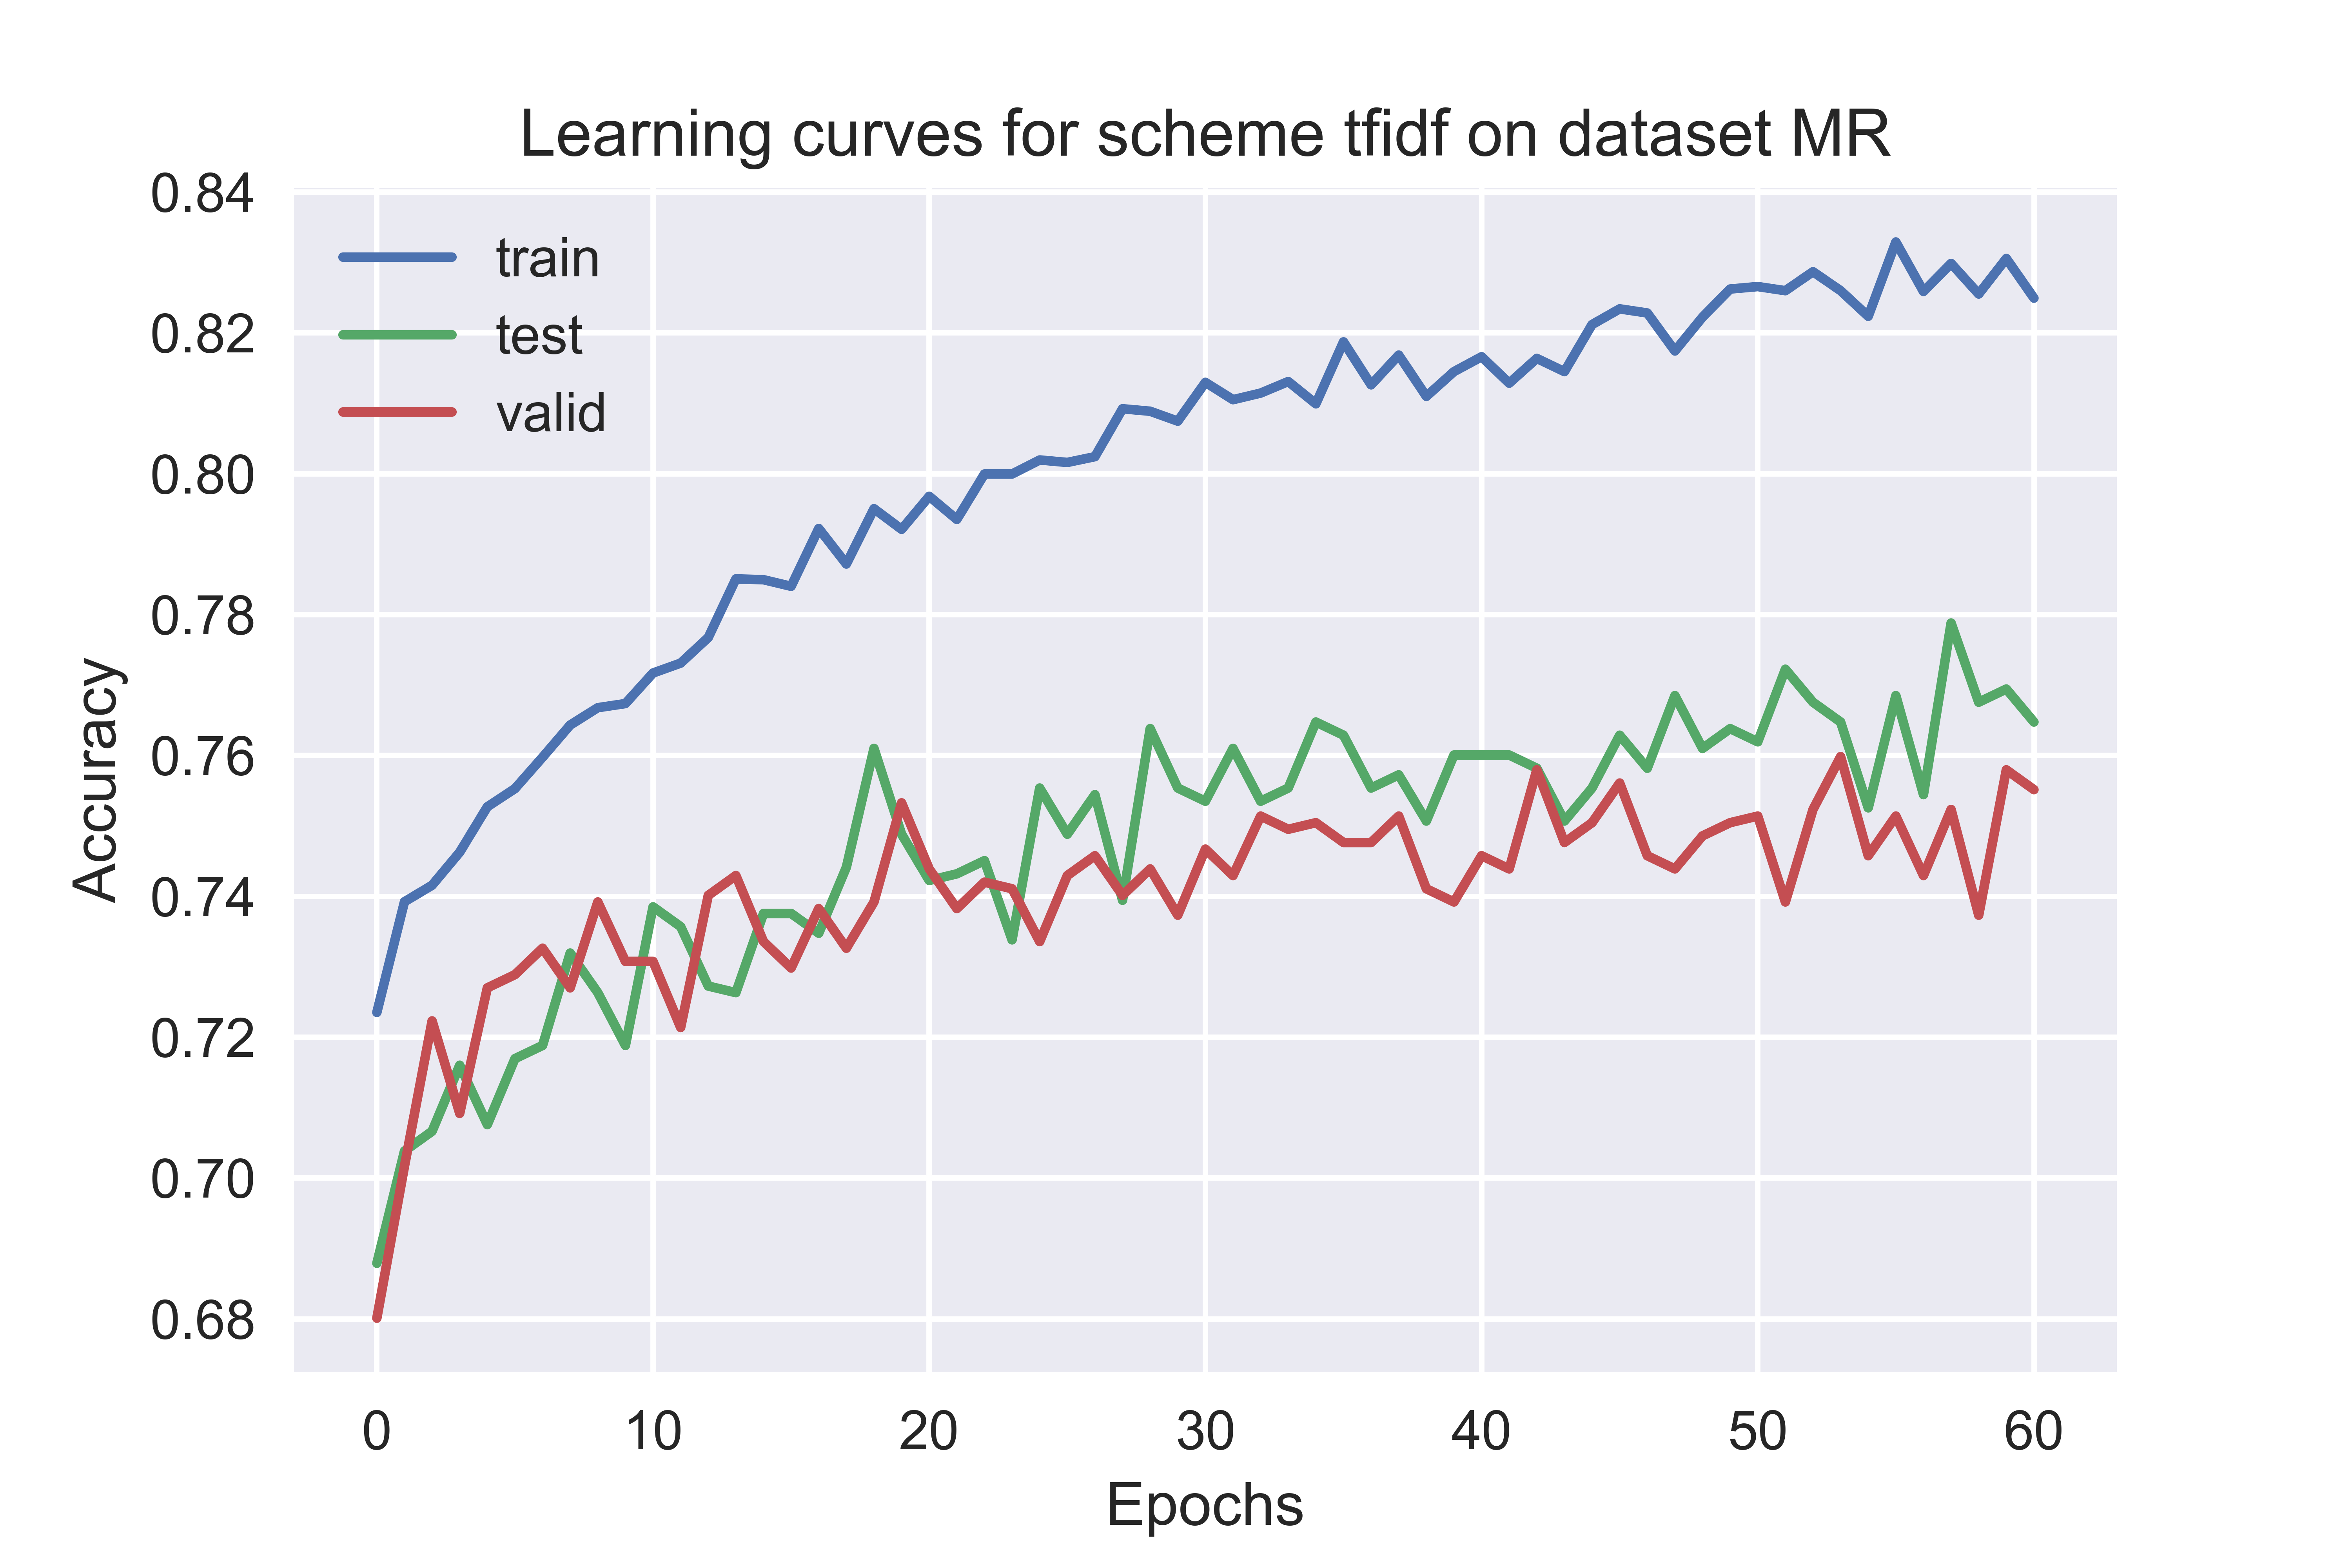
\includegraphics[width=0.8\textwidth]{images/learning_curve_MR_tfidf}}
    \caption[Learning curve for eLSA with tfidf weights on MR dataset]{Learning curve for eLSA with tfidf weights on MR dataset}
    \label{img:learning:curve}
    \end{figure}

    On figure \ref{img:learning:curve} we see a standard progress of accuracy through epochs. 
    We observe, that these curves are not entirely smooth as in batch gradient descent in neural networks.
    This is because we are not performing the exact gradient descent.
    The SVD part of eLSA is not deterministic and can be influenced by the weight $w'$.
    
    Recall from section \ref{sec:elsa:stopping} that we monitor the validation accuracy and stop the learning process when it plateaus. 

    \subsubsection{Multiple gradient steps}
    
    We perform an experiment, where we do multiple gradient steps on $w'$ for each loop. 
    This optimization routine is illustrated by algorithm \ref{algo:batch:multiw}.
    
    \begin{algorithm}[H]
        \KwData{$M$}
        \KwResult{trained $W$, $S$, $C$ }
        $w'^0 = 1$, $t=1$\;
        \While{performance is improving on validation dataset, $t$++}{
            recompute $S^t$ from $M \circ w'^{t-1}$\;
            compute embeddings $v^t$ from $M \circ w'^{t-1}$ with $S^t$\;
            fully train $C^t$ on $v^t$ and labels $y$\;
            \For{$0\leq i < m$}{
                update $W^t$: $w'^t = w'^{t-1} - \beta \frac{\partial E(C(S(M w'^{t-1}))}{\partial w'^{t-1}}$
            }
        }
        \caption{stochastic training of $w'$} \label{algo:batch:multiw}
    \end{algorithm}
    
    However this introduces another hyperparameter: number of performed $w'$ steps.
    We would like to to avoid new hyperparameters, so we do not spend too much resources on this experiment.
    Second problem with this approach is, that if we perform $m$ steps, the algorithm may be $m$ times slower. 
    This is a serious issue for $m>5$. 
    We perform experiments only for weighting scheme \texttt{None} with $200$ dimensional embedding and learning rate $0.1$.
    We perform $m=2$ and $m=5$ gradient steps and we present results in tables \ref{tab:multiw:notrec:2},
    \ref{tab:multiw:trec:2},\ref{tab:multiw:notrec:5} and \ref{tab:multiw:trec:5}.
    
    


\begin{table}[H]
\begin{center}

\begin{tabular}{lrrrr}
\toprule
{} &  CR &  MPQA &  MR &  SUBJ \\
\midrule
test  &  -0.01 &   0.00 &   \textbf{0.01} &   \textbf{0.01} \\
train &   0.02 &   0.00 &   0.01 &    -0.00 \\
valid &  -0.02 &   0.01 &  -0.01 &   0.00 \\
\bottomrule
\end{tabular}

\caption[Accuracy increase for 2 steps compared to 1 step]{Accuracy increase for 2 steps compared to 1 step}
\label{tab:multiw:notrec:2}
\end{center}
\end{table}




\begin{table}[H]
\begin{center}

\begin{tabular}{lrrrrrr}
\toprule
{} &  ABBR &  DESC &  ENTY &  HUM &  LOC &  NUM \\
\midrule
test  &     0.0 &     -0.01 &     -0.01 &     0.00 &    -0.01 &     \textbf{0.01} \\
train &     0.0 &      0.00 &      0.01 &     0.00 &     0.00 &     0.00 \\
valid &      -0.0 &     0.02 &     -0.00 &     0.01 &     0.00 &    -0.01 \\
\bottomrule
\end{tabular}

\caption[Accuracy increase for 2 steps compared to 1 step on TREC dataset]{Accuracy increase for 2 steps compared to 1 step on TREC dataset}
\label{tab:multiw:trec:2}
\end{center}
\end{table}




\begin{table}[H]
\begin{center}

\begin{tabular}{lrrrr}
\toprule
{} &  CR &  MPQA &  MR &  SUBJ \\
\midrule
test  &  -0.01 &   \textbf{0.01} &   \textbf{0.02} &   \textbf{0.01} \\
train &   0.03 &   0.01 &   0.01 &   0.01 \\
valid &  -0.02 &   0.01 &   0.00 &    -0.01 \\
\bottomrule
\end{tabular}

\caption[Accuracy increase for 5 steps compared to 1 step]{Accuracy increase for 5 steps compared to 1 step}
\label{tab:multiw:notrec:5}
\end{center}
\end{table}




\begin{table}[H]
\begin{center}

\begin{tabular}{lrrrrrr}
\toprule
{} &  ABBR &  DESC &  ENTY &  HUM &  LOC &  NUM \\
\midrule
test  &     0.0 &     -0.01 &     -0.00 &    -0.00 &     0.00 &     \textbf{0.01} \\
train &     0.0 &      0.01 &      0.01 &     0.00 &     0.01 &     0.01 \\
valid &     0.0 &      0.00 &      0.02 &    -0.01 &    -0.00 &     0.01 \\
\bottomrule
\end{tabular}

\caption[Accuracy increase for 5 steps compared to 1 step on TREC dataset]{Accuracy increase for 5 steps compared to 1 step on TREC dataset}
\label{tab:multiw:trec:5}
\end{center}
\end{table}



    We conclude, that making multiple gradient steps on $w'$ does not significantly nor consistently improve the accuracy and only makes the training process slower.
    The intuition, that multiple gradient steps on $w'$ may decrease the convergence time also showed to be wrong.


\begin{table}[H]
\begin{center}

\begin{tabular}{lrrrr}
\toprule
{} & CR & MPQA & MR & SUBJ \\
\$m\$ &      &       &      &       \\
\midrule
1  &     33 &      52 &     57 &      37 \\
2  &     32 &      43 &     45 &      46 \\
3  &     32 &      56 &     48 &      36 \\
4  &     33 &      68 &     63 &      39 \\
5  &     35 &      53 &     48 &      41 \\
\bottomrule
\end{tabular}

\caption[Number of needed training steps for different $w'$]{Number of needed training steps for different $w'$}
\label{tab:multyw:steps}
\end{center}
\end{table}


\begin{table}[H]
\begin{center}

\begin{tabular}{lrrrrrr}
\toprule
{} & ABBR & DESC & ENTY & HUM & LOC & NUM \\
\$m\$ &          &          &          &         &         &         \\
\midrule
1  &        32 &        38 &        38 &        72 &        38 &        48 \\
2  &        32 &        39 &        40 &        45 &        38 &        36 \\
3  &        32 &        48 &        35 &        38 &        32 &        38 \\
4  &        32 &        34 &        45 &        40 &        33 &        47 \\
5  &        32 &        37 &        36 &        32 &        37 &        52 \\
\bottomrule
\end{tabular}

\caption[Number of needed training steps for different $w'$ on TREC dataset]{Number of needed training steps for different $w'$ on TREC dataset}
\label{tab:multyw:steps:trec}
\end{center}
\end{table}

    The only relevant decrease in the number of required learning steps in tables \ref{tab:multyw:steps} and \ref{tab:multyw:steps:trec} can be seen for \texttt{TREC-HUM}.
    However this direction does not look very promising and we do not explore it further.
    }